\documentclass[a4paper,12pt]{report}
\usepackage{cmap} % Поиск PDF
\usepackage[T2A]{fontenc}  % Кодировка
\usepackage[utf8]{inputenc}  % Кодировка исходного текста 
\usepackage[english,russian]{babel}  % Кодировка исходного текста 
\usepackage{fontspec}
\usepackage{xcolor}
\usepackage{hyperref}
\definecolor{linkcolor}{HTML}{2d7ac7} % цвет ссылок
\definecolor{urlcolor}{HTML}{2d7ac7} % цвет гиперссылок
\usepackage{graphicx}
\graphicspath{ {./images/} }

\newcommand{\contractAddress}{0x37d29cb7d543300063a50d85389d409c01da7945}

\hypersetup{pdfstartview=FitH,  linkcolor=linkcolor,urlcolor=urlcolor, colorlinks=true}

\setmainfont{Ubuntu}
\providecommand{\versionnumber}{1.1}

% Title Page
\title{
\includegraphics[width=14cm]{logo}\\[2cm]Инфраструктура Portal Energy \\\normalsize v\versionnumber}
\author{Иванцов М. Мовчан П. Прусов М. Бутаков С. Патрикеев Б.}

\date{\today}


\begin{document}%
\maketitle
\tableofcontents
\clearpage


\chapter{Вступление}

Portal Energy была основана на слиянии технологий в сфере электроники, IT и Big data. Начиная с 2016 года, работаем над созданием недорогих и универсальных зарядных устройств для электромобилей. 

Тема электротранспорта позволила нам познакомиться и сформироваться в команду, однако, она не является единственной зоной нашего интереса. Со временем, по мере реализации всех поставленных целей, и достижению необходимых финансовых показателей, мы будем работать в сфере возобновляемой энергии, в социальной сфере, в сфере образования, в сфере интернета, и других. У общества много запросов, а у нас есть идеи, как эти запросы удовлетворить. 

Для превращения слов в конкретный результат, нам нужен эффективный инструмент. На наш взгляд эффективная система, работающая в рамках социума, немыслима без прямого участия представителей этого социума. Ведь именно люди являются носителями знаний о характере и нюансах наиболее актуальных проблем, и они же будут конечными потребителями результатов работы системы. Поэтому мы строим компанию, которая ориентирована, чтобы приносить пользу обществу и вовлекать людей в его развитие. Построить такую компанию и сделать её успешной - наша главная задача. 

В первую очередь, мы формируем сообщество заинтересованных людей, для которого Portal Energy -  инструмент.

Точкой старта развитие электротранспорта мы выбрали потому как в нашей стране эта тема находится на этапе зарождения, мы сами являемся её энтузиастами, и в долгосрочной перспективе здесь можно построить отличный фундамент для последующих проектов. 

Данный документ раскрывает наше видение развития электротранспорта в РФ, наши планы и их описание.



Ниже в тексте мы будем использоваться различные технические термины. Их краткое разъяснение дано в глоссарии. Если они вам знакомы, можете сразу переходить к разделу \ref{chapter3}.


\chapter{Глоссарий}

\section{Смарт-контракт}
Смарт-контракты похожи на классические контракты, за исключением того, что третьей стороной является множество людей, которые проверяют контракт на его исполнение и результат этого выполнения у всех участников должен совпадать, только тогда он будет считаться верным. В контракте мы можем прописать любые условия, которые надо выполнить. Из-за того что его выполняют множество участников, то мы не можем себе позволить исполнять очень сложные контракты, т.к. они будут требовать больших вычислительных мощностей. За вычисление берется комиссия в валюте ether(в сети Ethereum). После выполнения контракта сохраняется его состояние в блокчейне,
и удалить эту информацию невозможно.

\section{Блокчейн}
Выстроенная по определённым правилам непрерывная последовательная цепочка блоков, содержащих информацию. Простыми словами это цепочка блоков, каждый из которых обладает меткой времени, ссылкой на предыдущий блок и хранится на разных компьютерах.

\section{Криптовалюта}
Зашифрованный не регулируемый цифровой актив, использующийся в качестве аналога валюты в обменных операциях. Криптовалюта не имеет физической формы, она существует только в электронной сети в виде данных. Единицей такой валюты является «coin» (в переводе на русский –«монета»). При этом монета защищена от подделки, так как монета представляет собой зашифрованную информацию, скопировать которую невозможно.


\section{BNB}
Обменная единица Binance snart chain. Эта единица может делится на дробные части. Этой единицей может владеть как обычный кошелек, так и смарт-контракт. Такими же свойствами обладает и токен POE.

\section{Токен}
Единица учёта, не являющаяся криптовалютой, предназначенная для представления цифрового баланса в некотором активе, иными словами выполняющая функцию «заменителя ценных бумаг» в цифровом мире. Токены представляют собой запись в регистре, распределенную в блокчейн-цепочке.

\section{Токен Binance smart chain}
Надо написать про бинанс

Отличие токенов ERC-20 от других известных криптовалют, напри-
мер, биткоина или Litecoin, в том, что они привязаны к сети Ethereum, используют принятый внутри этой сети формат адресов и отправляются при помощи Ethereum-транзакций. Соответственно, транзакции с участием токенов ERC-20 можно прослеживать в обозревателе блоков.


\href{https://etherscan.io/address/\contractAddress}{Здесь} можно отследить движение всех наших токенов.

\section{Приватный Blockchain}
Все сети, такие как Bitcoin, Ethereum, EOS, являются публичными, т.к. любой анонимно может писать в эту сеть, из за чего пропускная способность сетей становится более ограничена, не всегда хочется публиковать какие то конфиденциальные данные в общую сеть, а также будет очень большая комиссия, если транзакция имеет тяжелый смарт контракт со сложной логикой, в общем мы имеем множество ограничений. Поэтому для бизнесса больше подходят приватные блокчейн системы, такие как Substrate (Polkadot фреймворк), Hyperledger Fabric, Hyperledger Sawtooth, Quorum и другие. За счет того что в сеть могут писать только авторизованные участники, которых мы все знаем. 

В результате мы имеем масштабируемую пропускную способность, отсутствие комиссий за транзакции. Единственные расходы которые несет бизнес - это на поддержку инфраструктуры, т.е. сервера и специалистов, которые занимаются поддержкой системы.



\chapter{Электромобили как технология}
\label{chapter3}
Мы уверены, что электромобили являются будущим автомобильной индустрии. Почему это так? 
В первую очередь, благодаря тому, что электродвигатель гораздо более эффективен, в сравнении с двигателем внутреннего сгорания (далее ДВС) (КПД электродвигателя 95-98\% против 38\% у ДВС). Что уже само по себе выливается в значительную экономию средств (заряжать электромобиль в 5-6 раз дешевле, чем обычный автомобиль, из расчета на 100 км). Плюс, электропривод экологичен, что для жителей мегаполисов крайне важно. Да и в целом, вопрос экологии становится всё более и более актуальным. 

Мы сделали небольшой обзор масштаба проблемы экологии в крупных городах, насколько грязным воздухом мы дышим, какие это имеет последствия и что нужно делать, чтобы ситуацию исправлять. Чтобы не утяжелять основной документ, здесь мы приводим ссылку на текст. Время чтения - 15 минут (\ref {https://docs.google.com/document/d/1Xvn2jIdGmjOemTvSG5J-kHtrBBC3f-odBOGnE6IfGFw/edit})

Кроме того, электромобили значительно манёвреннее и безопаснее обычных автомобилей, в связи с конструктивными отличиями. И наконец, потенциал электромобиля только начинает раскрываться, в то время, когда потенциал авто с ДВС уже достиг своего предела.

Однако возникает логичный вопрос - если электромобили лучше по большинству показателей, в разы дешевле в эксплуатации и зарядке, экологичны - почему тогда они массово не распространены в нашей стране? 



\chapter{Почему нет массового развития инфраструктуры в России?}
Вопрос действительно хороший. Чтобы вразумительно на него ответить, давайте посмотрим на страны, где электротранспорт уже распространён широко. 

\section{Электромобили в мире}
Лучше всего дела с электромобилями обстоят в Китае. В поднебесной за 2019 год было зарегистрировано более 1.2 млн новых автомобилей, а всего их 3.8 млн. Таже на начало 2019 года в Китае официально зарегистрировано более 1 млн зарядных станций.

На втором месте идут США. Там за 2019 год официально прибавилось 330 тыс. электромобилей. Всего в штатах их более 1.5 млн. штук, при этом зарядных станций там на 2019 год было более 200 тыс. штук.

В Европе, на конец 2019 года, количество электромобилей приблизилось к 2 млн штук, при проданных за год 550 тыс. штук и увеличении продаж в 1.5 раза в начале 2020 года.
Более того, дальнейшее будущее электротранспорта в развитых странах поистине безоблачно. 

Взгляните на графики роста выпуска электромобилей. Эти показатели говорят сами за себя. Стоит отметить, что в эту статистику входят не только абсолютные электромобили, но и подзаряжаемые гибриды (plug-in hybrids), т.к. подавляющее большинство из них имеют достаточно ёмкие батареи и полноценно используют зарядную инфраструктуру.
После 2023 года доля таких гибридов сокращается в пользу электромобилей.

Цифрами в перевёрнутых треугольниках обозначены некоторые из событий, ускоряющих смену автопарка на планете с ДВС на электро, либо являющихся важными контрольными точками этих изменений.

\vspace*{1cm}
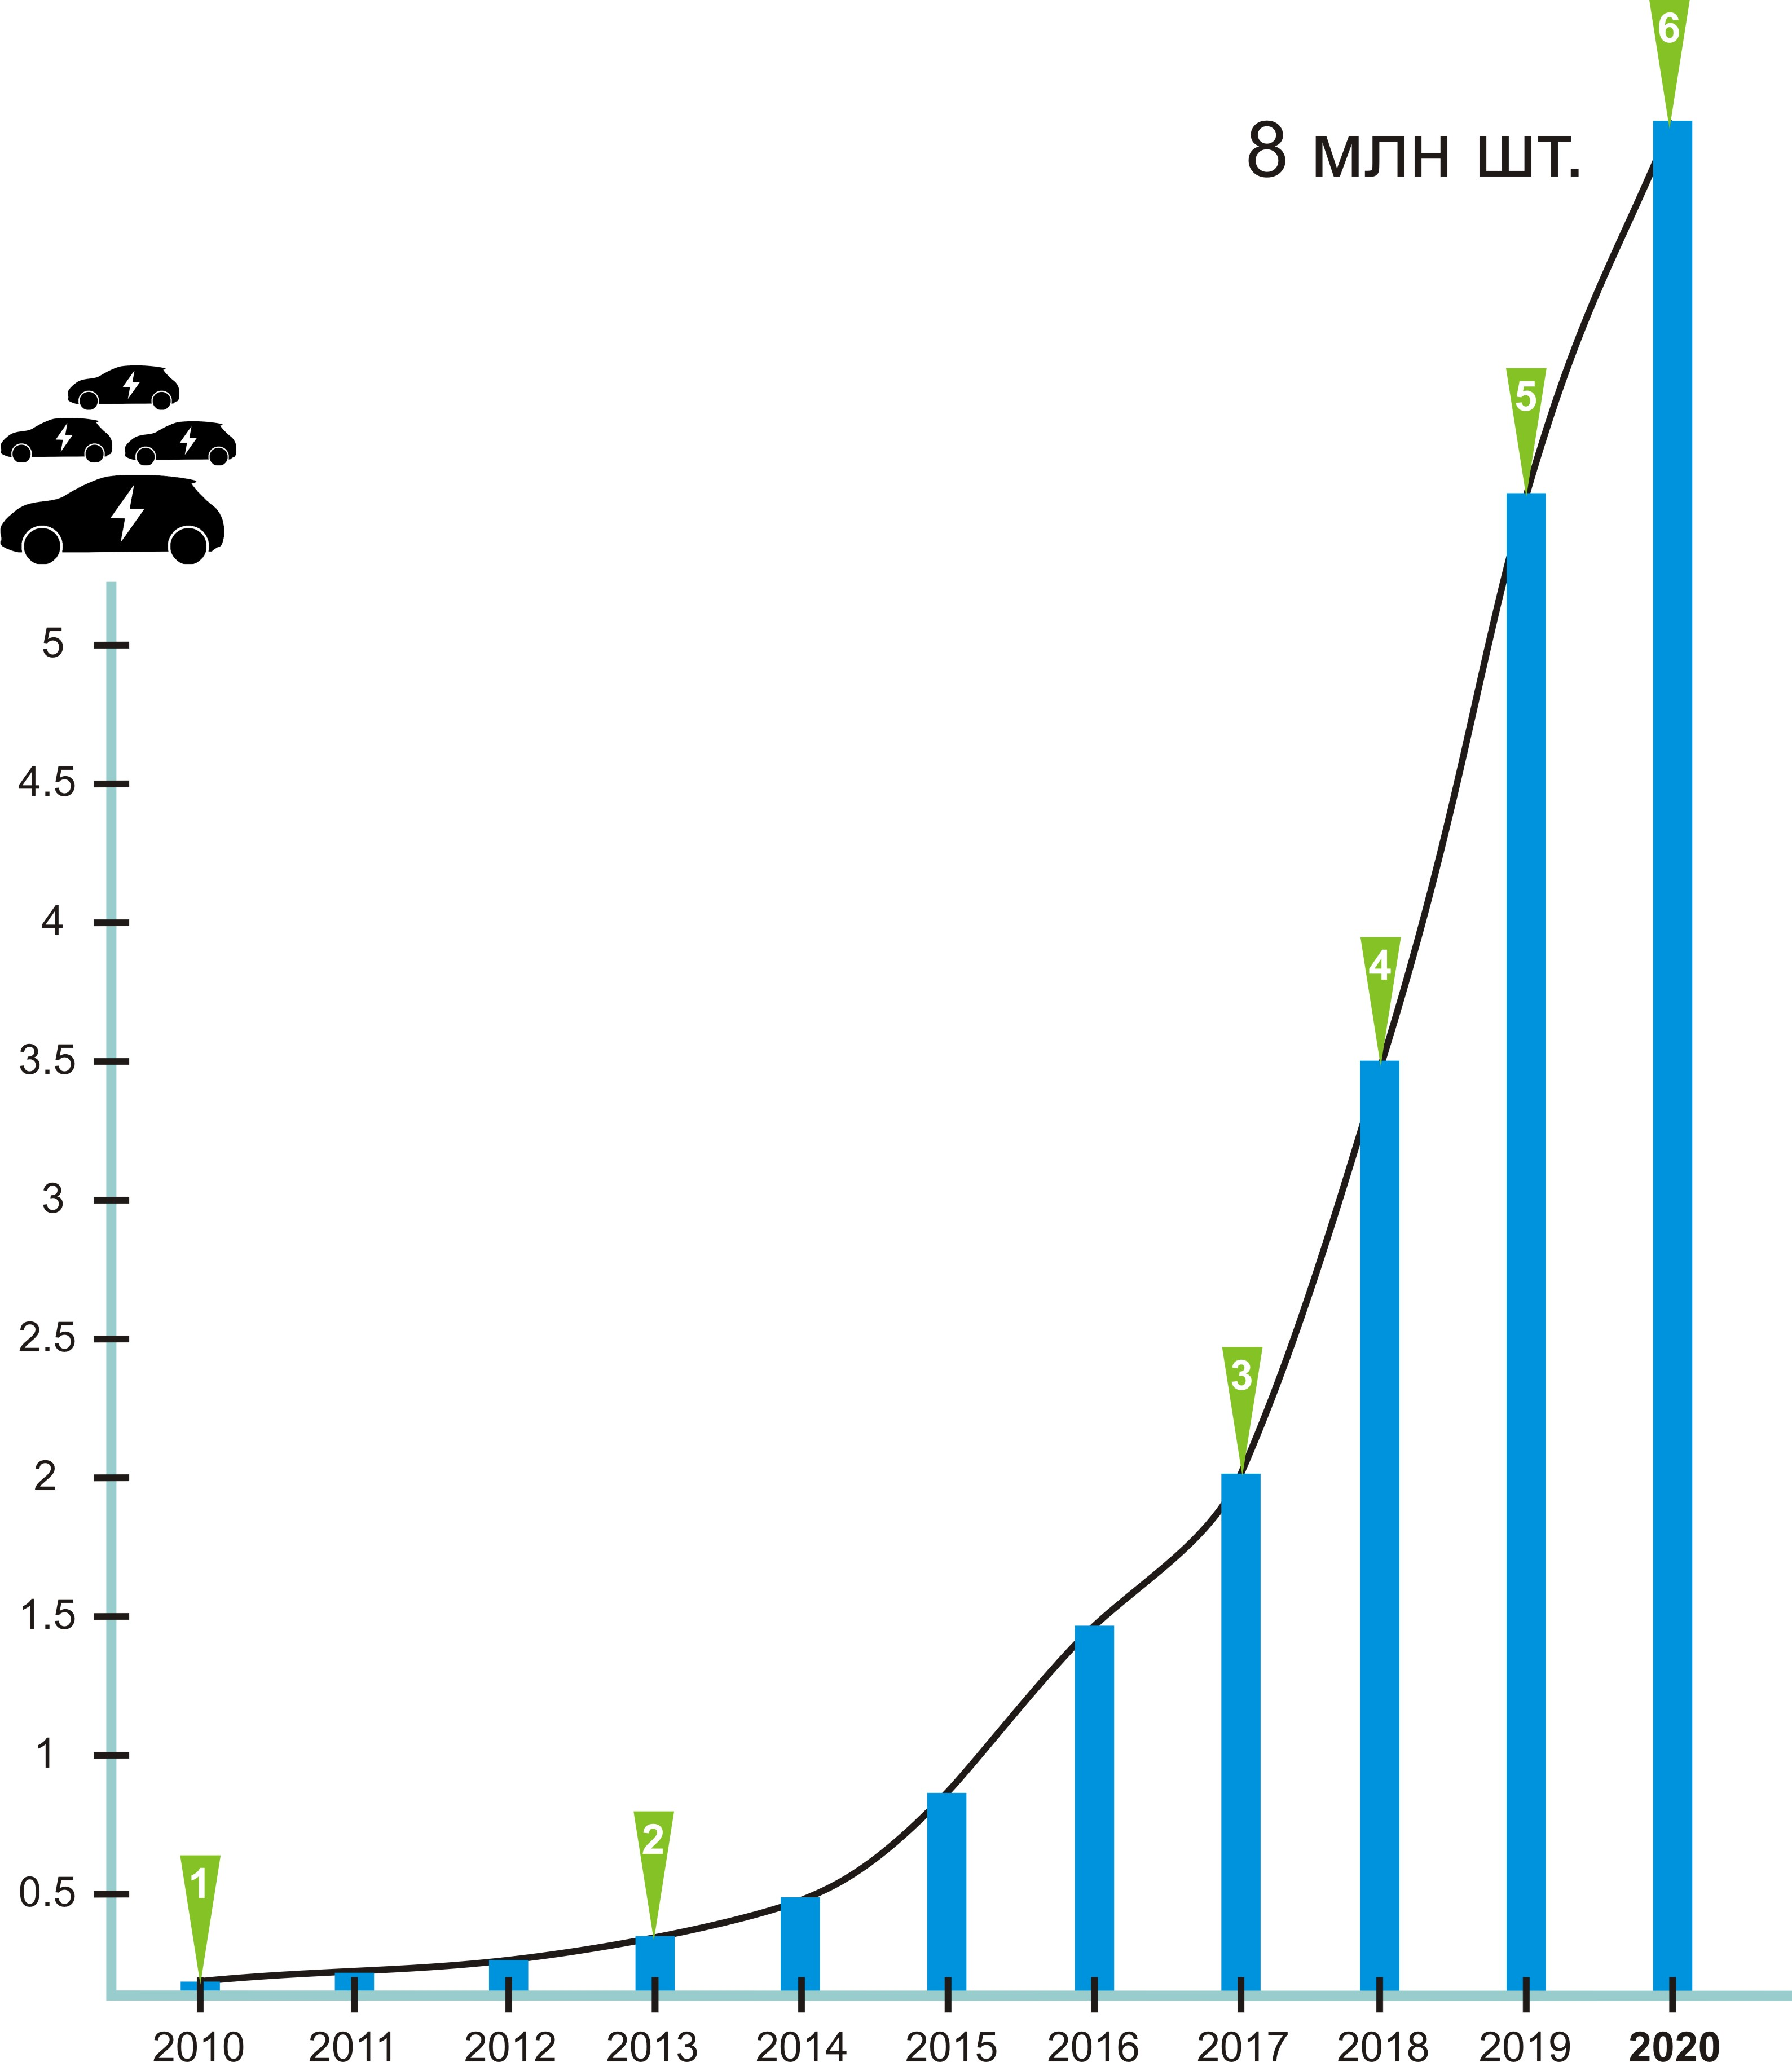
\includegraphics[width=12cm]{chart1}
\vspace*{1cm}

\begin{enumerate}
	\item Начало выпуска первого массового электромобиля в современной истории - Nissan Leaf
	\item Начало выпуска Tesla Model S
	\item Начало выпуска Tesla Model 3
	\item Каждый третий автомобиль в Норвегии электрический
	\item Количество зарядных станций в Европе превысило количество АЗС
	\item Количество проданных электромобилей Tesla превысило 1 млн штук
\end{enumerate}



\vspace*{1cm}
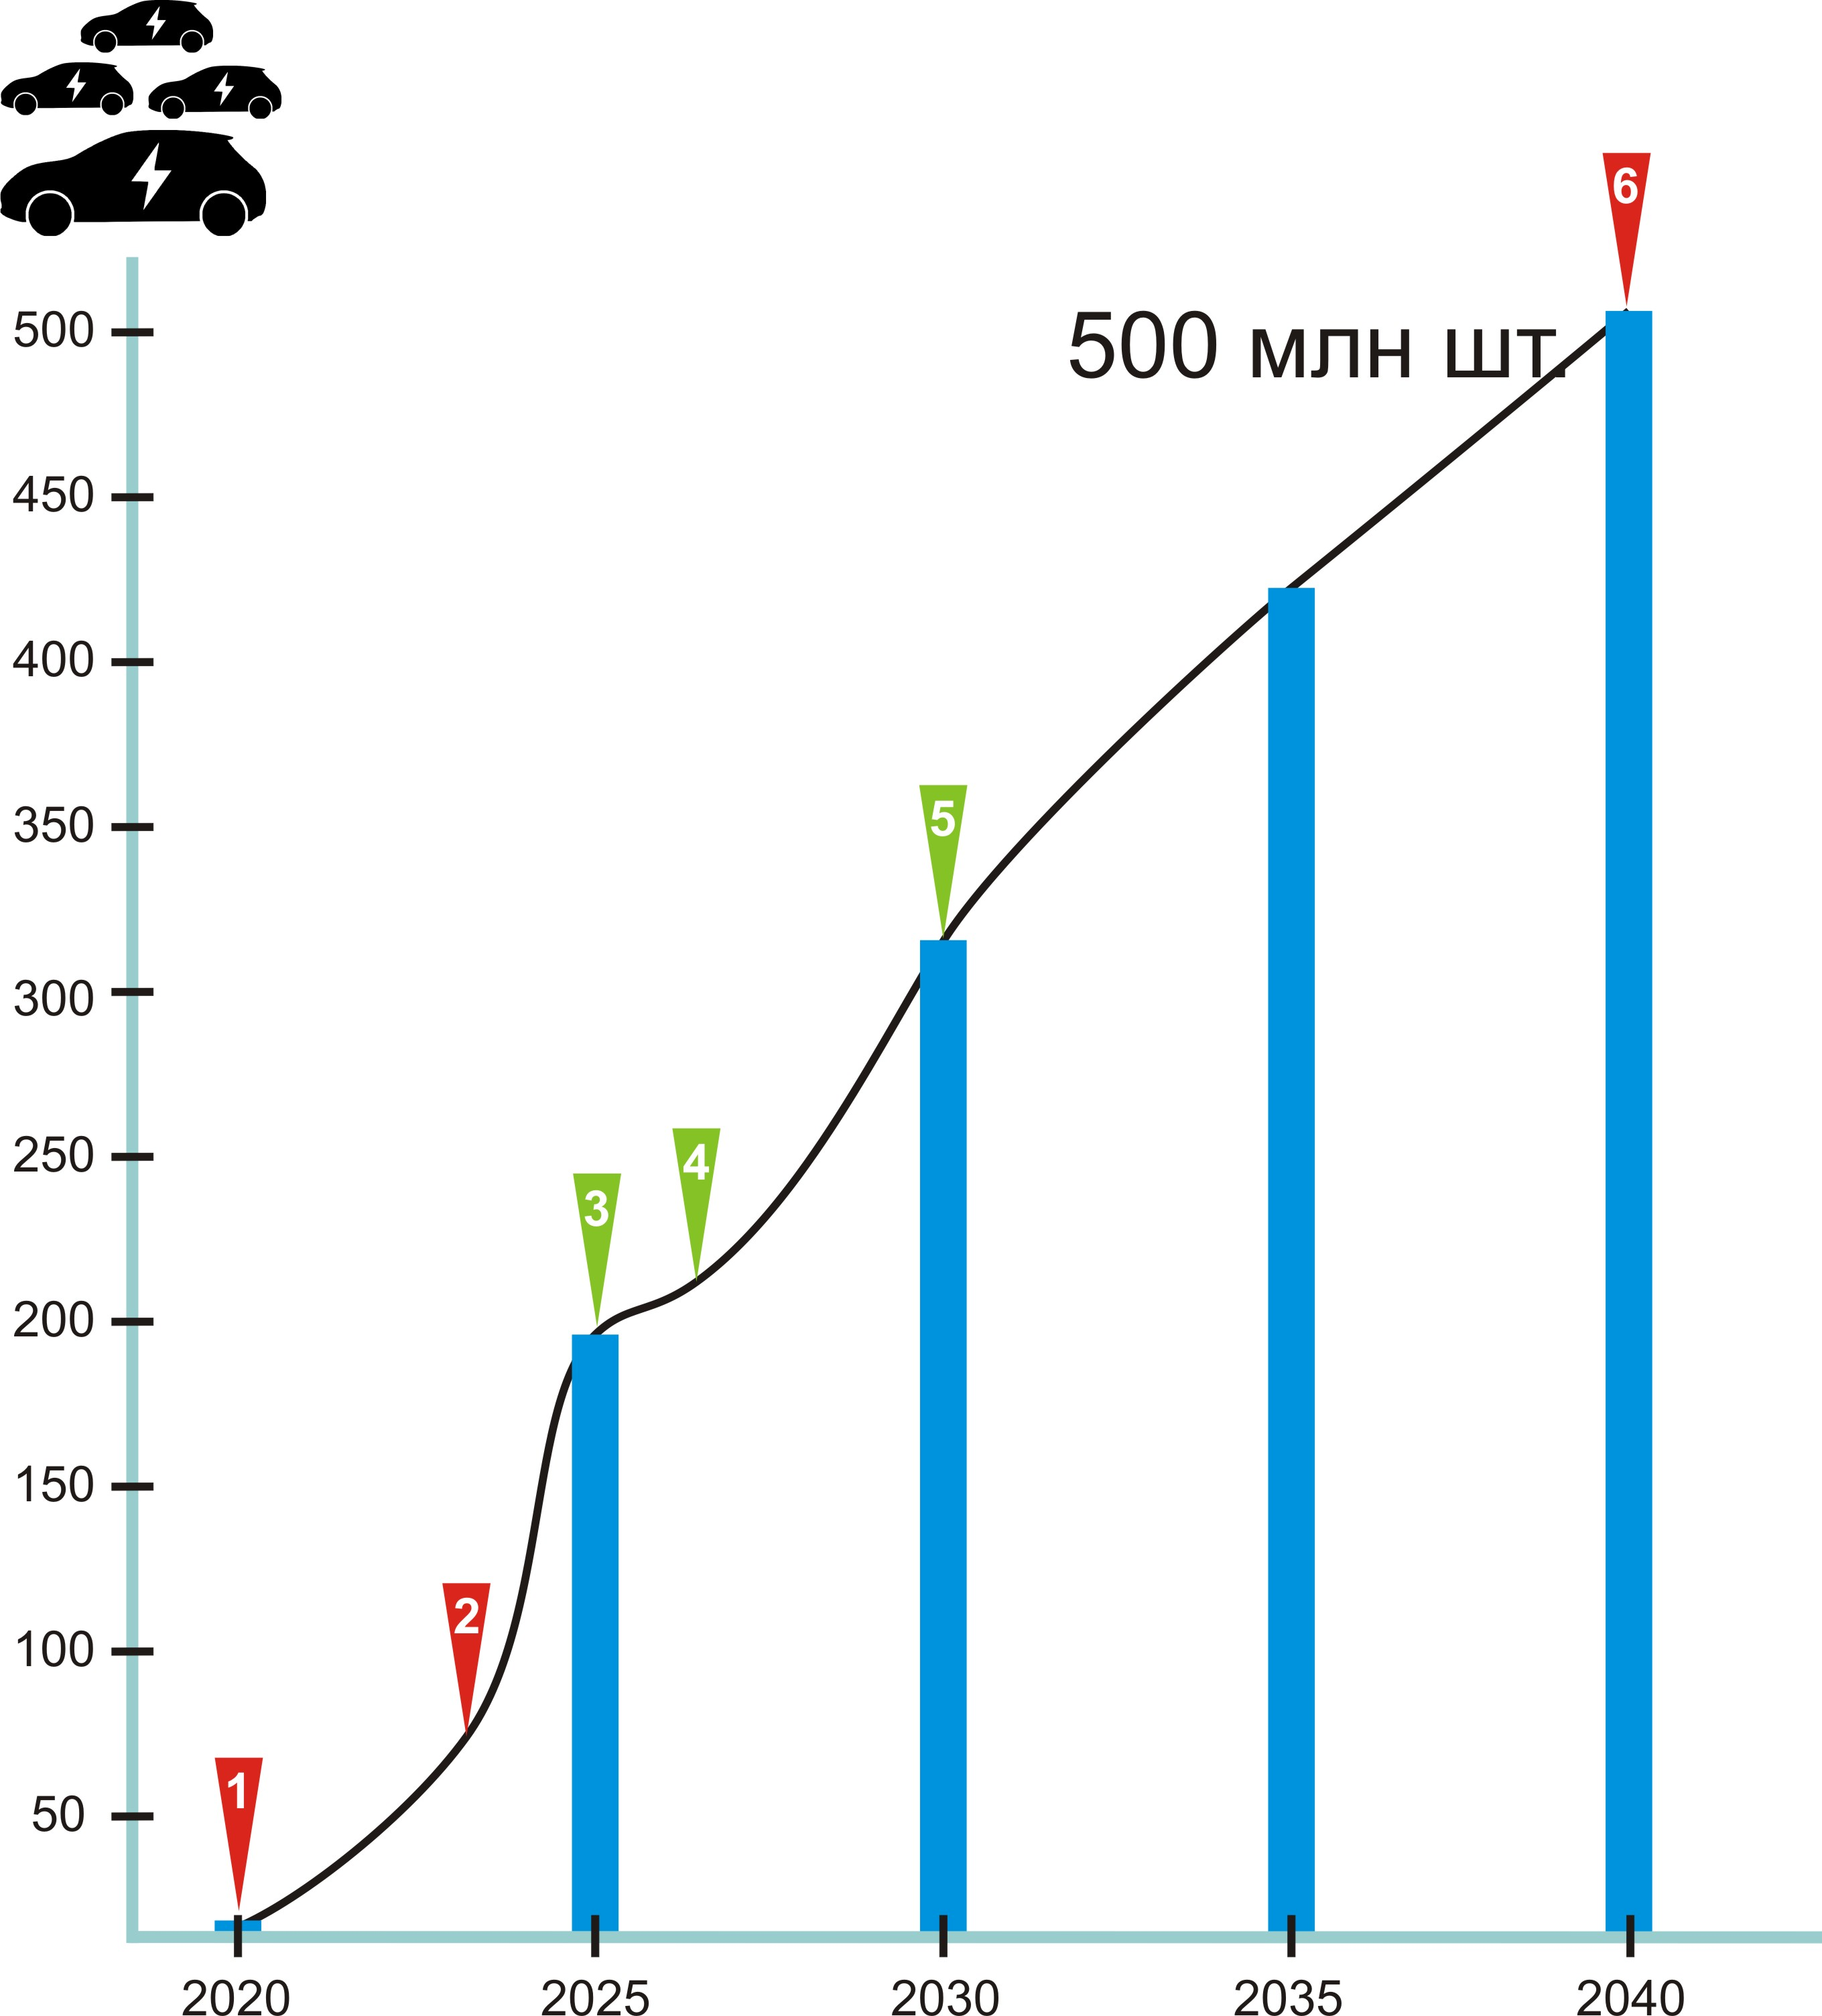
\includegraphics[width=12cm]{chart2}
\vspace*{1cm}

\begin{enumerate}
	\item Отказ от дальнейшей разработки в области ДВС крупнейших автопроизводителей, таких как BMW, Mercedes, Volvo, Audi, Volkswagen, Toyota
	\item Выравнивание стоимости электромобиля и автомобиля на ДВС (обусловлено снижением стоимости аккумуляторов)
	\item Начало распространения беспилотных, коммерческих электромобилей
	\item Toyota и Volkswagen прекращают выпуск автомобилей на ДВС
	\item Запрет эксплуатации ДВС в Голландии, Швеции, Шотландии, Дании и Израиле
	\item Полный запрет ДВС в Европе
\end{enumerate}


Какой вывод можно сделать из приведённых данных? В странах, где дела с электротранспортом обстоят хорошо, реализуются комплексные меры - развивается зарядная инфраструктура, создаются удобные приложения для владельцев электромобилей, принимаются поддерживающие законы, продвигается и активно обсуждается тема экологии. Во всех развитых странах полным ходом идёт переход на электромобили и со стороны производителей - сейчас каждый популярный бренд имеет в своём модельном ряду хотя бы один электромобиль.  


\section{Электромобили в России}
Сейчас в нашей стране всего около \textbf{500} полноценных зарядных станций. Чтобы понять, какое будущее ждёт электромобили при таком раскладе, нужно посмотреть на автомобили с ДВС через эту призму. Вы бы захотели приобретать авто, заправить которое можно было бы только в 500 точках на всю Россию? Которые, вдобавок, должным образом не обслуживаются, и внятных перспектив развития которых не предвидится. Наверное, нет. И это логично, поскольку автомобиль покупают не для самоистязания, а чтобы увеличить степень личной свободы и повысить комфорт передвижения. Поэтому неизбежным условием для увеличения количества электромобилей и их \textbf{комфортной} эксплуатации, является \textbf{развитие инфраструктуры}. 

\chapter{Проблематика инфраструктуры}
Помимо недостаточного количества самих станций, большинство из тех, что есть в нашей стране, расположены в самых странных и неудобных для автовладельца местах. А также не имеют должного обслуживания и адекватной информационной поддержки. В основном эти станции принадлежат гос. компаниям со всеми вытекающими.

Такое положение дел формирует “порочный круг”. Малое количество электромобилей делает идею развития зарядной инфраструктуры неинтересной для бизнеса. В свою очередь, отсутствие инфраструктуры значительно тормозит рост количества электромобилей. 

Решить проблему, по идее, способно государство, потому как у него достаточно ресурсов и инструментов. Наше государство пытается что-то делать (выпускаются законы, облегчающие финансовую нагрузку на владельцев электромобилей, адаптируются разрешительные акты, регулирующие установку зарядных станций, закупаются и устанавливаются бесплатные зарядные станции в городах и на трассах), но в масштабах страны эти усилия пока что незаметны. 

В 2016, когда мы только начинали, при слове “электромобиль” на нас смотрели, как на городских сумасшедших. И тогда действительно было рано для инвестирования в это направление по целому ряду факторов, главный из которых - рынка как такового еще не было. 

Однако сейчас рынок уже есть и самое время его осваивать.  


\chapter{Рынок России и перспективы бизнеса}
\section{Количество электромобилей}
Согласно данным аналитического агентства Автостат, в РФ количество зарегистрированных электромобилей в 2019 было 3.6 тысяч, в 2020 было 6.3 тысячи, и по данным Автоньюз, в 2021 почти 11 тысяч. По различным данным доля незарегистрированных электромобилей составляет еще от 25 до 40\% Данные для статей взяты из базы ГИБДД, поэтому мы можем считать их объективными. 

Тенденция роста почти 90\% в год, учитывая полное отсутствие инфраструктуры и пандемию.

Исходя из опыта общения с владельцами электромобилей и участия в огромном количестве различных мероприятий по теме, мы с уверенностью можем сказать, что количество потенциальных покупателей в десятки раз больше. Многие люди прямым текстом говорят: “когда появится возможность нормально эксплуатировать электромобиль, я сразу же его куплю”. Т.е. нас ожидает бум интереса к электромобилям, когда появится более-менее адекватная зарядная инфраструктура. 

\section{Потенциальный объём рынка зарядных станций}
Весь рынок РФ мы разбили на сегменты. Каждый сегмент мы рассматривали с двух позиций. Насколько вероятно в ближайшее время формирование потребности в станциях и потенциальный объём. 

\textbf{АЗС}

Со слов вице-президента НТС Дмитрия Гусева в РФ более 23 000 АЗС. 60\% из которых независимые. 

На АЗС целесообразно ставить только станции постоянного тока.

Мы пообщались с представителями всех крупнейших компаний на рынке по вопросу установки станций на их заправках. В целом, идея установки им интересна, и некоторые компании уже пробовали устанавливать станции и собирать статистику. Как только количество электромобилей увеличится, и станции станут рентабельными, они начнут ставить зарядные станции за свой счёт.


\textbf{Строительные объекты}

По данным Минстроя на февраль 2021 года зарегистрировано 3109 застройщиков, и выдано 5568 разрешений на строительство.

На 21 год запланирован ввод в эксплуатацию 40 726 тыс м2 - 796 000 квартир по всей стране. 

Согласно постановлению правительства РФ от 29.12.2009 необходимо обеспечивать минимальное количество парковочных мест 1.6 шт на 1 квартиру. Таким образом на 796 000 квартир, ожидаемых для ввода в эксплуатацию в 21 году, должно быть обеспечено 1273600 парковочных мест, и в соответствии с РДМ-32-28-2018 3\% из них должны быть оборудованы зарядными станциями для электромобилей (38 208 шт)

Из расчета на 1600 м2 1 станцию (из новой редакции петербургских Правил землепользования и застройки (ПЗЗ)), получается 25 454 станции по идее может быть поставлено в новостройках уже в 21 году.

\textbf{Гостиницы и отели}

Согласно данным Федерального агентства по туризму в России 14940 гостиниц и иных объектов размещения. 

Отели напрямую заинтересованы в установке станций, поскольку наличие такой станции уже сейчас даёт баллы в наиболее популярных приложениях букинга. 

\textbf{Трассы} 

Из соображений удобства рационально ставить 1 станцию постоянного тока каждые 50 км дороги. На трассах целесообразно устанавливать только сверхбыстрые (от 100 кВтт) станции постоянного тока. 

Всего протяженность трасс, где в принципе имеет смысл размещать зарядные станции  - 63 290 км (1265 шт)

\textbf{Малый и средний бизнес, торговые точки, бизнес-центры}

Владельцы любых коммерческих помещений могут покупать зарядные станции и с помощью приложения монетизировать. По сути станция будет работать, как вендинговый аппарат, генерируя небольшую прибыль с продажи электричества, как рекламный щит (модели с экраном) привлекая электромобилистов, и тем самым повышая продажи основных услуг бизнеса. 

Как видно, с увеличением количества электромобилей, нас ожидает бум интереса к зарядным станциям. 

Зарядная инфраструктура и электромобили являются частями одного целого, и рассматривать их отдельно не имеет смысла. И соответственно, усилия наиболее целесообразно вкладывать сразу в обоих направлениях.  

Сценарий развития рынка вполне очевиден. 

Увеличение количества различных моделей электромобилей и их удешевление (за счет конкуренции и развития аккумуляторной химии) с одной стороны и постоянное и неизбежное подорожание бензина с другой, будут стимулировать темпы прироста количества электромобилей. 

Растущую потребности в зарядных станциях всё больше будет привлекать компаний и частных предпринимателей к развитию инфраструктуры. Точечно поставленные станции будут генерировать всё большие прибыли, и их количество будет неизбежно расти. 

К определенному моменту количество зарядных станций достигнет точки, когда эксплуатация электромобилей станет в целом удовлетворительной, и на первый план в принятии решения о переходе на электротранспорт выйдет экономическая выгода от его использования. Информация об этом распространится в инфополе и всё больше людей начнут задумываться о покупке электромобиля.

Это резко увеличит потребность в электромобилях. На растущий спрос рынок ответит ростом предложения. Всё больше компаний начнут заниматься привозом и продажей электромобилей. 

Рост оборота капитала рано или поздно привлечет в сферу электротранспорта крупных игроков, и начнется масштабное развитие по всей стране.

Чтобы иметь адекватные шансы на конкурентную борьбу с крупными компаниями, к моменту, когда пойдёт ажиотаж нужно уже быть полностью готовыми: иметь качественный продукт, налаженное производство, отлаженную логистику и средства коммуникации с клиентом и приличный доход. 

Ждать, когда произойдёт взрыв и только потом начинать - значит остаться у обочины и наблюдать, как рынок съедают корпорации.

Рынок будет сформирован и полностью занят. Это неизбежность технологического развития общества. Открытым остаётся вопрос - какие конкретно игроки успеют зайти на этот рынок и получить долю. Мы уже в их числе. Тоже хотите? Тогда добро пожаловать в сообщество. 

Однако, сказать, что мы получим свою долю рынка - это одно. А вот реально её получить - совсем другое. Для того, чтобы слова превратить в результат, нужно понимание что делать, необходимые инструменты и люди, которые сделают то, что нужно. 

\chapter{Стратегия освоения рынка}
\section*{Подготовительный этап}
\textbf{Продукт}
Любой бизнес начинается с качественного, конкурентоспособного продукта. 

Один из наших основных продуктов - это услуга по зарядке электромобилей. Для реализации практической функции - непосредственной зарядки автомобиля - нам необходимо соответствующее техническое устройство - зарядная станция. 

Поскольку потребитель нашего продукта человек, помимо технических характеристик, важным свойством зарядной станции является дизайн. Наш дизайн - это одно из конкурентных преимуществ, роль которого будет возрастать по мере развития рынка и появления всё большего количества производителей. Станция должна выглядеть стильно, аккуратно и привлекать внимание. 

Другое свойство, обязательное для конкурентоспособного продукта, это удобство взаимодействия. Наша задача сделать практическое использование станций интуитивно понятным, комфортным и стабильным. Для этого мы разработали мобильное приложение. Также в долгосрочной перспективе приложение это мощнейший инструмент коммуникации с пользователями и соответственно серьезное конкурентное преимущество. Приложение уже можно скачать для Android и IOS. Функционал будет расширяться и в конечном итоге приложение станет одним из ключевых инструментов внутренней коммуникации, объединяющим все наши продукты.

Услуга по зарядке электромобилей - продукт комплексный и сложный. Чтобы на выходе получилось необходимое качество, все его элементы должны быть созданы профессионалами и должны управляться профессионалами.

\textbf{Команда}

На момент Августа 21 года, команда Portal Energy составляет 19 человек (выросла с 7 человек). У нас есть:
Команда управления, 
команда инженерной разработки, 
команда разработки софта, 
производственная команда,
команда дистрибуции. 

Количество человек будет расти по мере увеличения количества задач. 

Как уже говорилось, Portal Energy это сообщество заинтересованных людей, что значит, любой член сообщества является частью команды. Мы рассчитываем привлекать участников сообщества к деятельности компании, когда для этого будут разработаны необходимые инструменты.

\textbf{Независимость и гибкость}

В современном мире производство, как правило, распределено. Крупнейшие компании закупают компоненты у разных производителей и уже из них собирают свой конечный продукт. 

Мы, разумеется, тоже рассматривали данную модель. Но быстро от неё отказались. Специфика российского рынка делает международную логистику крайне дорогой и уязвимой к накладкам по времени. Что мы позволить себе не можем, потому как в случае с перебоем комплектующих мы сразу же нарушаем все договоренности по срокам с клиентами. В долгосрочной перспективе с такой уязвимостью рассчитывать на успех в конкурентной борьбе, как минимум, наивно. (upd из Марта 2022 - ох, как же проницательно было это решение! :) ) 

Второй вопрос - это вопрос гибкости. Разработка технологических устройств предполагает длительную отладку и постоянное усовершенствование определенных узлов и элементов. Оперативно получить необходимые комплектующие для тестов имея поставщика за океаном - невозможно.

Таким образом мы пришли к неизбежности собственной разработки всех комплектующих и написания софта. 

На сегодняшний день мы сами разрабатываем платы контроллеров, сами пишем для них ПО. Мы сами производим корпуса и производим сборку станций. Единственные звенья, которые пока что являются импортом - коннекторы и инверторы. Однако, и их производство мы ближайшее время наладим на территории России. 

\section{Этап отладки и подготовки к масштабированию}
\textbf{Производство}
Итоговый вариант производства, который мы хотим видеть - производство полного цикла. На вход поступает металлопрокат и комплектующие электроники, на выходе получается полностью готовая к работе зарядная станция. 

Такое производство мы будем создавать в два этапе. 

Первый этап - экспериментальная лаборатория с малой производственной мощностью - до 50 станций в месяц. 
Второй этап - производство полного цикла с мощностью от 1000 станций в месяц. 

На текущий момент мы полностью реализовали производство первого этапа с мощностью 40 станций в месяц и перспективой её приращения до 100 штук в месяц. Производство расположено рядом с офисом разработчиков, что позволяет нам комфортно и оперативно реализовывать изменения и исправлять ошибки, найденные в станциях, поступивших в эксплуатацию.

Второй этап мы начнём, когда весь запланированный модельный ряд будет отлажен и инфраструктурный проект будет способен загрузить производство хотя бы на 100 + станций в месяц. И постепенно наращивать мощность.

Таким образом к моменту начала ажиотажа мы планируем иметь производство с мощностью от 1000 станций.

О старте привлечения инвестиций мы сообщим на наших информационных ресурсах. Поэтому если вам интересна идея инвестирования в производство, следите за новостями. 


\chapter{План развития инфраструктуры}
Сейчас в инфополе нет никакой активности вокруг темы электротранспорта, и у людей, которые являются нашими потенциальными клиентами, сформировано однозначное понимание - в России зарядной инфраструктуры нет и не предвидится. Поэтому первая задача - сформировать интерес к теме электротранспорта, создать движение информации и показать Portal Energy, как авангард в вопросе развития зарядной инфраструктуры.

Это сформирует у людей запрос на покупку электромобилей. Поскольку сейчас купить хороший электромобиль по адекватной цене в России практически невозможно, наша вторая задача - удовлетворить спрос на электромобили. Для этого мы уже общаемся с различными производителями электротранспорта и прорабатываем процесс доставки на территорию нашей страны. 

Рост количества электромобилей сформирует потребность в увеличении количества зарядных станций. Т.е. наши потенциальные клиенты станут реальными. И следовательно, третья задача - удовлетворить спрос на зарядные станции.

Наш инфраструктурный проект - это работа над всеми тремя задачами. 

В первую очередь необходим инструмент эффективной совместной деятельности. Portal Energy является таким инструментом. 

Дальше нужен производитель, который смог бы удовлетворить потребность будущей инфраструктуры в самих станциях и взять на себя задачи по их обслуживанию. Portal Energy является таким производителем.

Также немаловажным фактором при развитии инфраструктуры электротранспорта, является понимание его специфики. Модель поведения владельца электромобиля отличается от модели поведения владельца авто с ДВС. Местоположение АЗС обусловлено техническими ограничениями, поэтому они всегда находятся, в первую очередь там, где можно физически построить такую станцию и адекватно её обслуживать. Владелец авто с ДВС неизбежно привязан к локации заправки и для него это обязательная “боль” с которой он вынужден мириться. 

Что же касается зарядной станции для электромобиля, она может находиться там, где это реально будет удобно для автовладельца, потому как требования к пространству для установки станции незначительны. И, поэтому, при разработке карты местоположений станций, необходимо опираться в первую очередь на местоположение владельцев электротранспорта. И только в этом случае заправка автомобиля сможет перестать быть неизбежной головной болью владельца, а станет простым, понятным и не напряженным нюансом в эксплуатации автомобиля. Он будет заряжаться не где-то во время дороги, а пока владелец будет заниматься своими делами, поскольку в каждом удобном месте под рукой всегда будет зарядная станция.

Также важно, чтобы вокруг зарядной станции (в особенности так называемоей "медленной", т.е. станции переменного тока) была специфическая инфраструктура. Сеанс зарядки электромобиля на медленной станции, как правило, длится от 2 часов. Соответственно, это время владелец должен иметь возможность провести не только в салоне своего электромобиля. В крупных городах наиболее рациональными местами для начала развития инфраструктуры являются районы проживания электромобилистов. Далее по приоритету идут крупные экономические объекты (торговые центры, бизнес-центры и т.д.) от которых уже будут тянуться нити зарядных станций дальше по городу. Между городами, расположенные через каждые 50-100 км станции постоянного тока, смогут полностью снять проблему подзарядки электромобиля в длительной поездке. 

Именно такой мы видим логику развития инфраструктуры.


\vspace*{1cm}

\chapter{Формат взаимодействия с сообществом}
Поскольку подобная задача может быть решена только в условиях абсолютного доверия участников сообщества друг к другу, мы обязаны были это доверие сформировать. По нашему мнению, лучшим фундаментом в формировании доверия является полная прозрачность всех финансовых процессов в организации. И для обеспечения такой прозрачности, мы выбрали \textbf{блокчейн}. 

Схема работы простая. Мы производим станцию, находим место, которое обладает необходимыми характеристиками и производим установку. Далее мы эмитируем токены в количестве соответствующем затратам на производство и установку станции. После этого токены могут быть выкуплены. Далее цикл повторяется. Но только до момента, пока сеть не выйдет на уровень доходности, позволяющий устанавливать новые станции без продажи токенов. Подробнее об этом в разделе про эмиссию токена. 

 
Весь доход от станции будет распределятся между участниками. При этом участники не привязаны к конкретной станции, а получают доход со всех установленных станций в системе, тем самым имея диверсифицированный портфель. Это позволит сгладить разницу между популярными и менее популярными локациями. 
Более подробно смотрите раздел \ref{capital} распределение дохода.

В итоге мы имеем инструмент который позволит более быстро и коллективно построить зарядную инфраструктуру с прозрачной и безопасной системой финансов.

По мере создания инфраструктуры, мы планируем развиваеть сообщество и привлекать владельцев токенов к различным активностям. Более подробно об этом мы расскажем в отдельных материалых, когда проект будет говтов. На сегодняшний день 

\section{Токен}

Токен имеет адрес - \contractAddress 

В нашей системе мы используем токены, созданные с помощью Binance smart chain, которые называются \textbf{POE}. Основная их функция - выражать в цифровом формате зарядные станции, которые мы устанавливаем. Именно потому что они выражены материальными объектами, они имеют определённую начальную стоимость.

Приобретая токены, вы становитесь владельцем (собственником) части зарядной инфраструктуры. (Объём собственности соответствует вложенным средствам). В свою очередь, объекты инфраструктуры являются не просто физическими объектами, в результате работы они производят дополнительную стоимость, за счёт того, что люди используют их для зарядки автомобилей. В результате этого, в структуру будут постоянно поступать реальные деньги, которые мы будем тратить на обслуживание станций и распределять между собственниками (держателями токенов) в качестве прибыли. Способность токена генерить доход является вторым фактором, влияющим на стоимость. Таким образому, у токена, помио рыночной цены, будет и реальная стоимость. Это важно, поскольку реальная стоимость никогда не сможет упасть ниже определённого значения, сформированного объективными условиями. 

Мы выбрали Binance smart chain, потому что данная сеть является крайне устойчивой и безопасной и в ней низкая комиссия за транзакции. Но больше, конечно, из-за стоимости транзакций. :)
Для реализации токена мы использовали открытую разработку \\ (\href{https://openzeppelin.com/}{https://openzeppelin.com/}), которае прошла проверку на аудит безопасности многими крупными компаниями, что гарантирует безопасность нашего токена.


\subsection{Эмиссия и распределение токенов}

Токен имеет формально неограниченную эмиссию. Но "майнить" его можно только через установку реальных станций. Что фактически делает эмиссию ограниченной, поскольку невозможно бесконечно устанавливать зарядные станции - рано или позжно закончится место, и значит, не будет возможности и эмитировать новые токены. Более того, мы планируем прекратить выпуск токенов под установленные станции, когда сеть будет приносить достаточную прибыль, чтобы из фонда обслуживания можно было непрерывно финансировать дальнейшее развитие. 

Такая модель для нас наиболее удобна, поскольку мы не ограничены фиксированной эмиссией, и с другой стороны, объективная невозможность бесконечной эмиссии, защищает систему от бесконечного размытия долей и инфляции. 

 
Адрес токена:
\textbf{0x8eA9a18A98E5cDbE93cacEa82Ea3e9c2CB8Dc520}

Купить токен можно (дописать).  

42.8\% от выпускаемых токенов идёт на счёт компании для покрытия сопутствующих расходов на установку и обслуживание станций.

Как это будет выглядеть в цифрах.

Мы произвели и установили зарядную станцию. Весь проект стоил 4 600 \$ Мы считаем необходимое количество токено по текущему курсу (на момент написания данного текста - 1.2 \$). Это получается 3 500 POE. 42.8\% (1498) при этом зачисляется на счет компании. После этого токены можно купить.

\textbf{ВАЖНЫЙ МОМЕНТ!} Для того, чтобы токен начал приносить прибыль, его нобходимо "застейкать", т.е. разместить на адресесе смарт-контракта распределения. Застейканные токены будут генерить прибыль в размере равном соотношению объёма токенов у владельца и общего числа застейканных токенов. 

Посмотрим на примере.

Пусть человек владеет 2000 POE. Он решил застейкать 1000 POE.

На момент принятия такого решения общий стейк был равен 99 000 POE. Соответственно с добавление еще 1000, общий стейк стал равен 100 000 POE
Пусть сеть получила 1 000 000 рублей прибыли за отчетный период. Поскольку доля токенов человека от общего объёма стайка равна 1\%, то доход, который он получит будет равняться 1\% от 1 000 000 а именно - 10 000 рублей. Важно понимать, что 1000 POE, не участвовавшая в стейке не, принесет никакого дохода. 


\subsection{Фонд развития и поддержки}
Для того чтобы поддерживать уже созданную инфраструктуру и развивать текущую без вливания новых инвестиций создан кошелек: 
\textbf{0xe09a4e0DEC6365C8f8f58Ca5C14eE2706EA541Dc}

На этот кошелек будет попадать процент от дохода станций, на момент старта это 20\%, этот процент потом можно будет менять путем голосования держателями токенов. 


\subsection{Доходность системы }
\label{capital}

Доходность всей сети зависит от того, сколько стоит киловатт энергии, продаваемой через станции и количества проданных киловатт. 

Также важно учитывать, что одна и та же станция может генерировать разный доход. Это зависит от места, где станция расположена.

Формула расчета годового дохода простая:


\textbf{X * Y * Z * A} 

Где:

\begin{itemize}
  \item Х - стоимость киловатта (имеется в виду чистый доход, т.е. тариф станции минус тариф энергокомпании)
  \item Y - сколько киловатт может продать станция в час (Переменный ток: коннектор тип1 - 9, коннектор тип2 - 22. Все наши инфраструктурные станции оборудованы обоими коннекторами, т.е. минимальное  количество - 9, максимальное 31. Постоянный ток - заявленная максимальная мощность. Т.е. 40, 60, 80 и т.д. Если подъезжает несколько машин, мощность распределяется равномерно и не может превышать максимальную)

\item Z - количество часов, которое станция работает в сутки (может быть от 0 до 24)
\item A - количество рабочих суток в году

\end{itemize}

Средняя прибыль на киловатт, на которую мы ориентируемся,  5-8 рублей на станциях переменного тока и 8-15 рублей на станциях постоянного тока. 

Чтобы система была интересна инвестрам, мы решили поставить минимально возможный объём доходности сети. Он формируется из рассчёта, что 1 станция переменного тока в среднем генерит не меньше 22.5 кВт в день, и прибыль с киловатта не меньше 5 рублей. Таким образом получается, что минимально возможный доход 1 станции в год - 41 062 рублей. 

При средней стоимости проекта, включающего производство станции, поиск и подготовку места, установку и пусконаладку, в 400 000 рублей, мы гарантируем минимальную доходность в 10\% годовых. Может быть больше, но меньше - нет.


По станциям постоянного тока цифра будет другая. Её мы уточним, когда начнём ставить в сеть станции постоянного тока.


Вся статистика по фактически проданным киловаттам каждой станцией доступна в режиме реального времени на нашем сайте. 

\section{PortalChain}

\vspace*{0.5cm}

\includegraphics[width=13.6cm]{substrate-logo}
\vspace*{0.5cm}


Помимо обеспечения безопасности, ключевым требованием к системе является финансовая прозрачность.
Именно поэтому нами был выбран Substrate Framework для создания собственной приватной сети PortalChain.

Поскольку сеть Ethereum не позволяет экономно проводить большое количество транзакций, а также может быть временно нагружена и принимать транзакции долго и с динамической комиссией за транзакцию, что для нас неприемлемо, то для реализации бухгалтерии мы создадим свою приватную сеть, используя готовое решение.

\textbf{Substrate Framework} - это блокчейн платформа для создания своих блокчейн сетей, которая позволит эффективно вести систему бухучёта для всей зарядной инфраструктуры, обладает высокой скоростью обработки транзакций, а так-же как и любой блокчейн невозможностью подделать реестр.

Еще одно \textbf{преимущество} приватной сети, в том, что мы можем давать разным ключам разные уровни доступа. Читать из сети смогут все, а писать в эту сеть смогут только зарядные станции которые имеют приватный ключ для подписи транзакции на оплату использованной энергии.

Держатели от \textbf{5000} токенов получат возможность стать валидаторами транзакций в нашей блокчейн сети если они того пожелают, для того, чтобы система была еще более безопасной и устойчивой к внешнему вмешательству. Так же наш блокчейн будет обладать копиями всех реальных документов которые будет заключать компания с другими организациями, например договор тарифного плана на электричество для конкретной зарядной станции.
Каждый обладатель токена может запросить нотариально заверенную копию любого документа, заведенного в систему.

В заключение, мы хотим сказать, что прекрасно понимаем масштаб и сложность нашей цели, и понимаем, что нечто подобное можно реализовать только вместе. Сообщество единомышленников - это не какая-то абстрактная конструкция, это реальные люди, включая и тебя тоже. Поэтому, если ты готов принять непосредственное участие в изменении окружающей тебя действительности, вступай в сообщество Portal Energy.

\section{Присоединяйтесь}

\begin{itemize}
	\item Telegram канал - @portal\_energy
	\item \href{https://www.youtube.com/channel/UCtPxyCkz73i78F9HChlO61w}{Youtube}
	\item \href{https://www.instagram.com/petr_roadrunner/}{Instagram}
	\item \href{https://portalenergy.tech}{Сайт}
\end{itemize}

\textbf{По всем вопросам пишите в Telegram - @portal\_alexey}

\end{document}          
